\section{Introduction}

The end of classical device scaling means that the power per unit area on chip
is rising with each technology generation.  This implies that architectures for
future technology nodes will not be able to power-on all components of the chip
simultaneously, with some estimates being 50\% ``dark silicon'' by
8nm~\cite{isca11:dark-silicon}, which is less than 10 years away.  This trend,
the utilization wall, will curtail expected performance improvements.
Interestingly, much of the core's energy is not expended in the functional
units, but rather in the power-hungry structures needed for
attaining reasonable performance on general purpose workloads.  To exploit this,
architects have in part turned to hardware specialization and
accelerators, which sacrifice generality for efficiency in executing either
specific computations or computations for certain application domains.

Though accelerators hold great promise, with many new accelerator designs
showing significant efficiency and performance gains, the research and 
insights have been fragmented.  Newly proposed accelerators are evaluated 
in their own toolchain, generally with a specific general purpose core, and with 
a set of chosen benchmarks.  Solving this by integrating tens of accelerators 
into a single simulation system and developing compatible compilers 
for them is intractable due to development time.  This means that attaining 
insights into accelerators which transcends specific simulators, core design
points, evaluation metrics and applications is extremely difficult.
This limitation hinders our ability to understand the future of acceleration 
in terms of their behavior, design and use.
%benefit, and how can we do it?

%insights into how the applications and choice of 
%general-purpose core affects what is the best accelerator 
%to apply is very difficult.  Also, this lack of information hinders our ability
%to see what are the future opportunities for acceleration: where can we get more
%benefit, and how can we do it?

Going forward, the architecture community needs a methodology for modeling
acceleration which is detailed and accurate, yet simple and abstract, to help
unify and improve the current understanding.  With such a
tool, we can begin to address the biggest challenges of acceleration:  First,
we must understand where the biggest benefits of acceleration could come from,
and what are the biggest limitations, so we can best focus our efforts on
problems which will push the limits of their effectiveness (\emph{Finding
Accelerator Limits/Opportunities}).  Second, we need a strategy for designing
accelerators which can explore a broad range of the possible space in a short
amount of time (\emph{Effective Practices for Accelerator Design}).  Finally,
we need practical and flexible ways to employ multiple accelerators at
runtime so that the promises of accelerators can be achieved in a
wide variety of domains (\emph{Enabling Practical Multi-Acceleration}).

In pursuit of these challenges, this dissertation proposes 
a novel abstraction called the Transformable
Dependence Graph (TDG), which can model certain important forms of acceleration.  
It is designed to accurately capture interactions between the accelerator, general
purpose core, and application at sub-instruction granularity.   The core idea is to
represent the program’s execution trace as a dependence graph of
micro-architectural events, and to perform transformations on this
representation to model various forms of acceleration.  This concept is based
on the dependence-graph of Fields \emph{et
al.}~\cite{fields:isca01,Fields:2002:SMP:545215.545222}, and our contribution is
in showing how graph transformations can model acceleration.

\subsection{Completed Work}
Completed work has shown that our model and implementation is accurate in
capturing both the out-of-order execution of processors, as well as the
transformation from OOO dependence-graph trace to model four different classes
of accelerators.  Our results have shown that, using the dependence-graph model, we can
achieve an average error of less than 15\% in both performance and energy
reduction for all classes of accelerators we target. In general, there are
certain accelerator classes which can be modeled accurately, discussed in
detail in Section~\ref{sec:scope}~(Page~\pageref{sec:scope}).  
The flexibility, accuracy, and high-abstraction of the TDG is useful for 
solving a variety of problems beyond just modeling, 
and forms the basis for the proposed research.  

%The TDG can be used for purposes beyond modeling, and this proposed
%work is described next.

%Using the TDG we have three primary research directions.  First, we
%aim to understand what are the limitations and opportunities with
%currently proposed accelerators.  By formalizing architectural
%optimizations as graph transformations, we can quickly explore the
%potential of an architecture.  Second, we can use the TDG to help design
%new accelerators.  By finding applications which are not exploited by
%current accelerators, we can use this insight to develop next generation
%accelerators which are complementary to existing designs.  Also, the
%abstract nature of the TDG enables rapid design space exploration, and
%by associating transformations with units of hardware, we may be able to
%partially to fully automate this process.  Finally,  if multiple
%accelerators can provide high benefits, then we will need practical ways
%of scheduling them.  We will explore how to use dynamic execution
%information along with performance/efficiency goals to schedule
%accelerators.

\subsection{Summary of Proposed Work}

%By employing the TDG as an efficient modeling tool, my proposed work addresses
%the aforementioned accelerator challenges.
Figure~\ref{fig:proposed-work-overview} gives a high-level overview of each
proposed work compared to the current approaches for each problem, 
and they are outlined below.

\begin{figure}
\vspace{-.2in}
\begin{adjustwidth}{-0.3in}{-0.3in}
  \begin{center}
    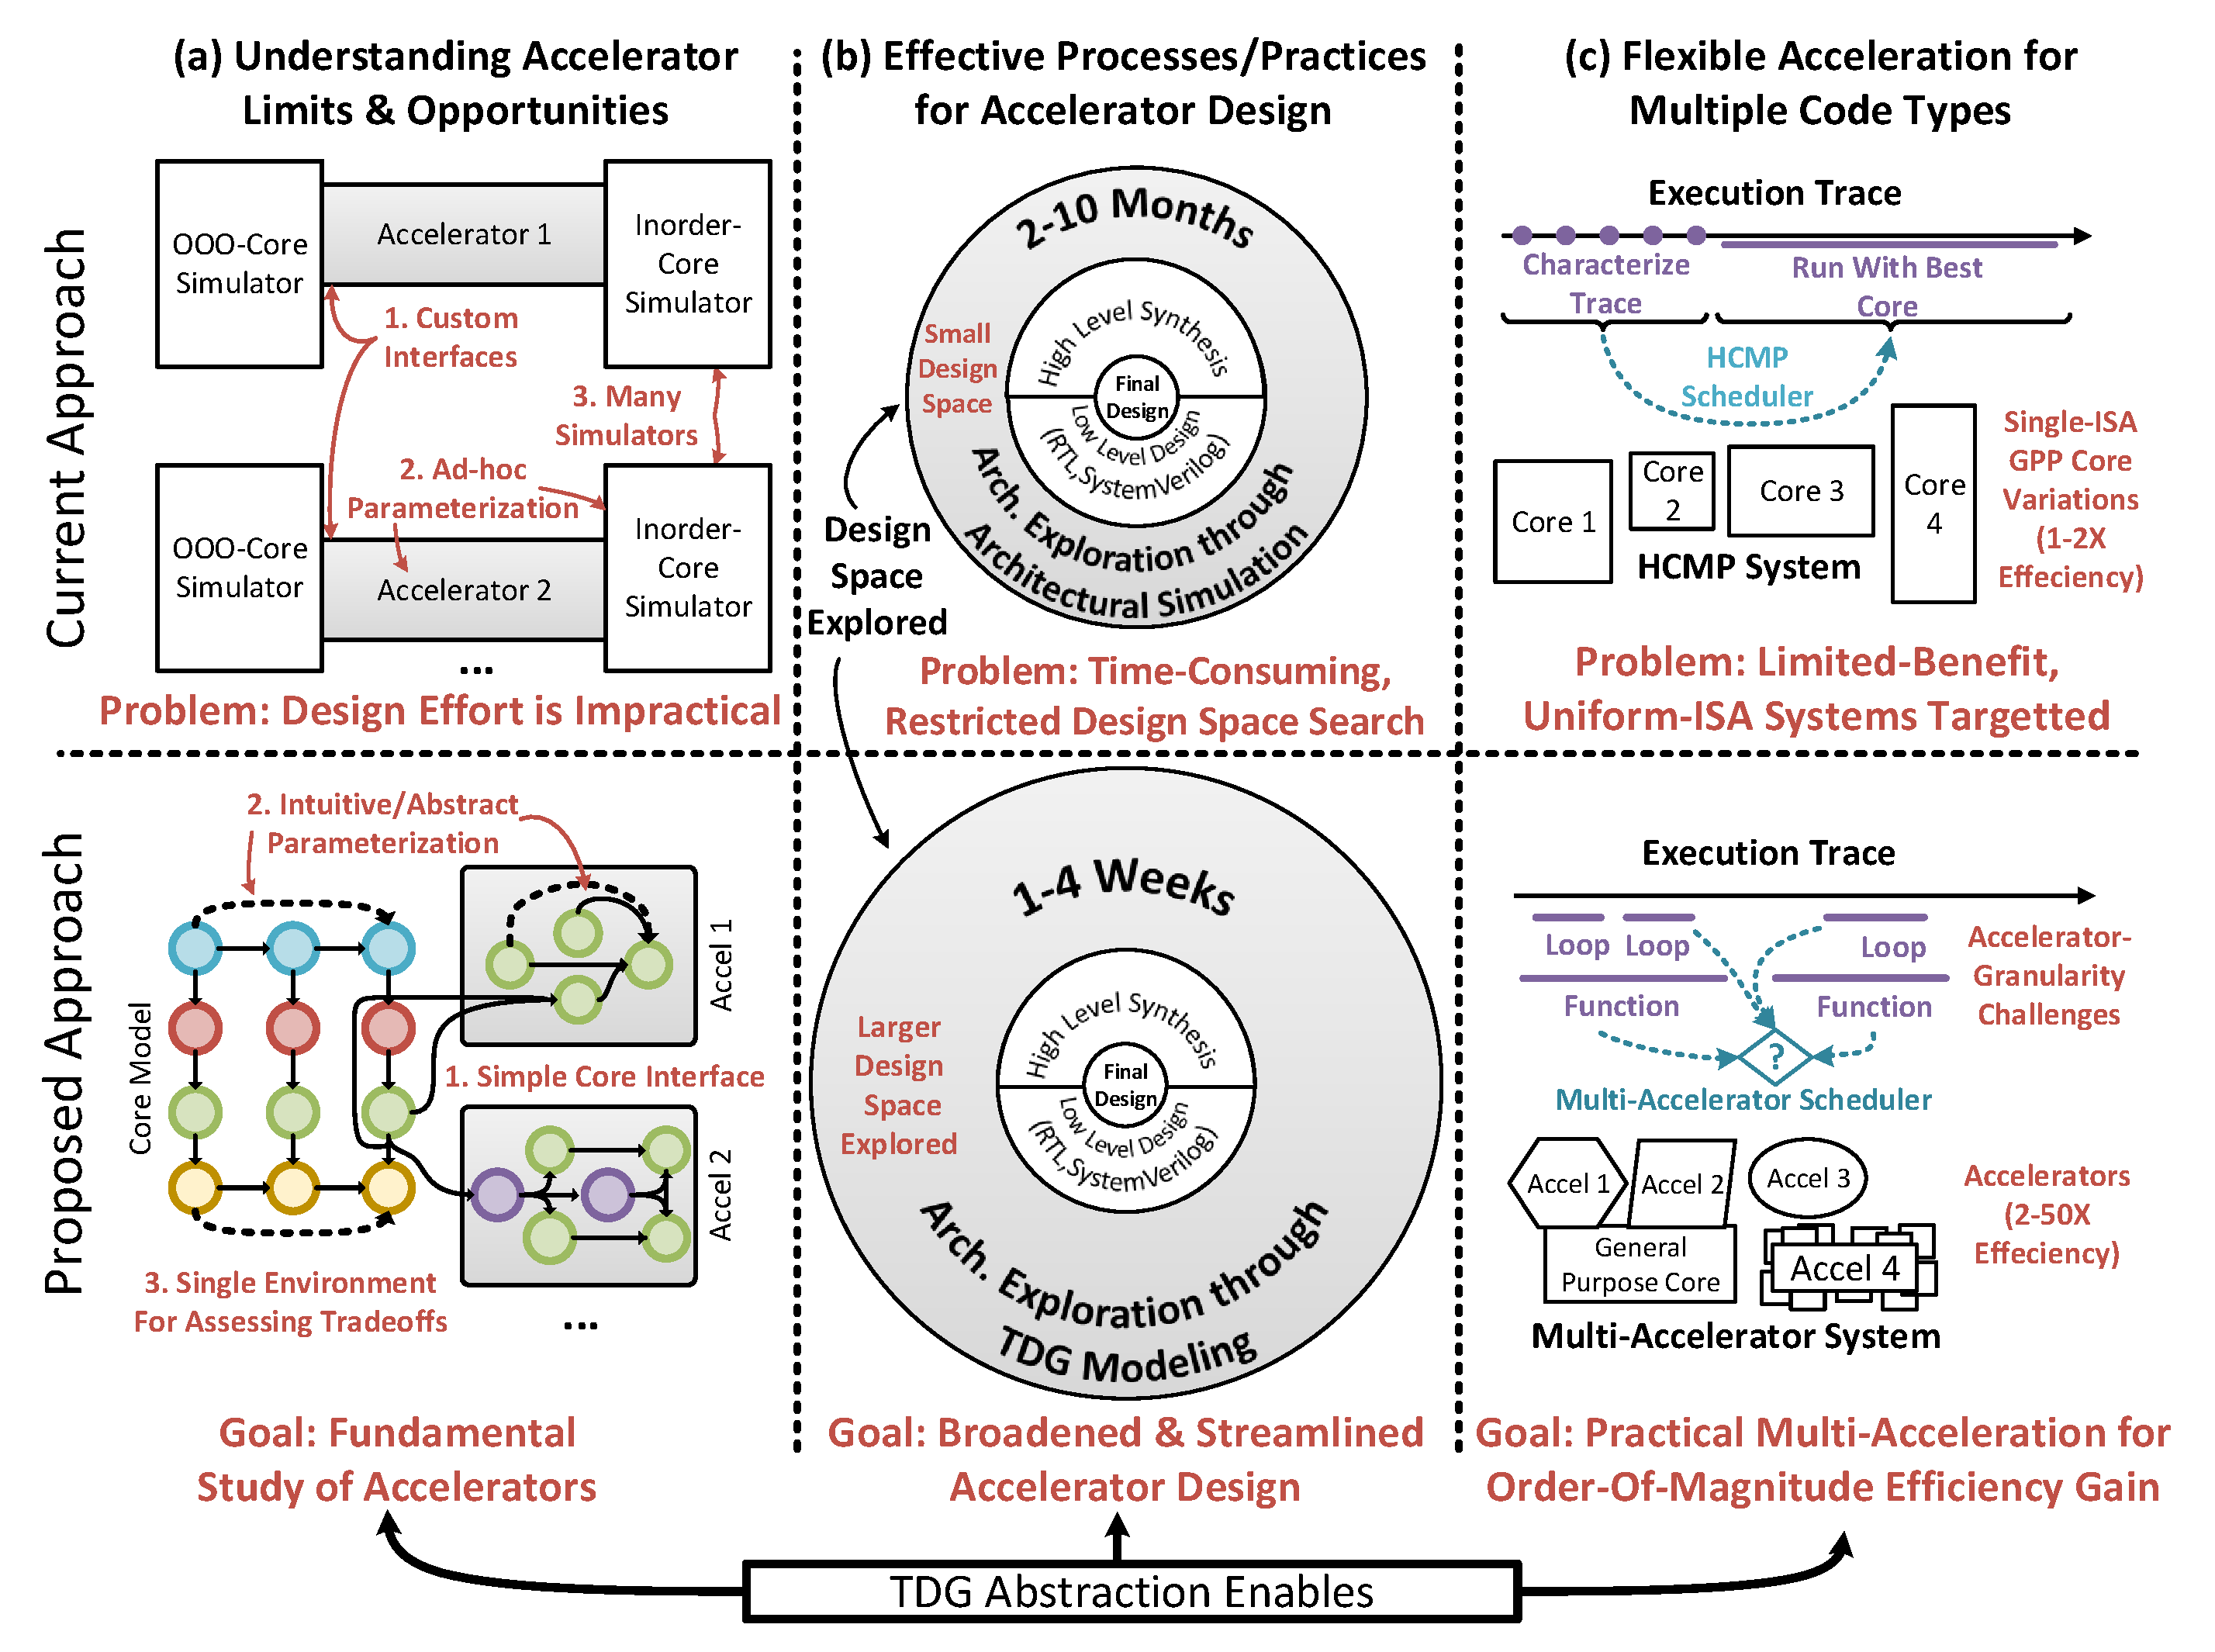
\includegraphics[width=1.0\linewidth]{figs/proposed-work.pdf}
  \end{center}
\vspace{-0.2in}
  \caption{Summary of proposed work as compared with current best techniques.}
  \label{fig:proposed-work-overview}
\vspace{-0.05in}
\end{adjustwidth}
\end{figure}


\begin{itemize} \item \textbf{Limits and Opportunities of Acceleration:} For the
future of acceleration, it is important both to understand the fundamental
limitations of accelerators, as well as to know where the largest benefits can
come from.  We can better understand accelerators by modeling hypothetical
designs which break current limitations, and observing their new behavior.
Current approaches using simulators would be too tedious because they require
ad-hoc accelerator implementation and integration with multiple simulators. The
proposed approach employs the TDG to simplify modeling and unite the modeling
of accelerators under a common framework, making the study of their nature
consistent and practical.  This work's goal is to uncover the fundamental
limitations of accelerators, to show what are the most important challenges for
future accelerator architects.


\item \textbf{Effective Processes/Practices for Accelerator Design:} Existing
accelerator design strategies are ineffective because they rely on tedious
simulator modeling, consider accelerators in isolation, and inappropriately bin
applications to accelerator designs.  Overall, they are able to cover less of
the design space, and require more design time.  To address this, this research
proposes an accelerator design strategy which leverages the TDG.  Primarily, it
presents a higher level of abstraction, both broadening the explored design
space while hastening the process.  The unified framework makes it simple to
compare with existing accelerators during the design-space exploration, which
can help prune the design space quickly.  Also, many TDG models can be used
together to find the regions with the biggest potential for new accelerators,
giving insight to architects without the need to bin accelerators.  The
research so far shows how to use the TDG to help design an accelerator for
nested loops, a contribution on its own.

\item \textbf{Enabling Flexible/Practical Multi-Acceleration:} 
By employing multiple accelerators in a single system, it is possible to achieve
flexible efficiency for a variety of code types.  Current approaches lack the
ability to target systems more general than uniform-ISA heterogeneous architectures.
To attain the benefits of multi-acceleration, it is
necessary to partition regions of applications onto the most beneficial
accelerator.  This decision can be complicated, because
accelerators are only legal on different granularities of code.
Also, certain accelerators can have serious drawbacks if applied on the wrong
application regions.  The proposed research is to explore static
and dynamic mechanisms, including intuition-guided static approaches, 
compiler-generated TDG-based prediction, multi-granularity sampling techniques, 
and machine-learning based performance/energy models.  

\end{itemize}

\subsection{Relation to My Previous Work}

The inspiration for this dissertation topic stems from my previous work in creating
a unifying general framework for spatial architecture scheduling~\cite{ILP_Sched},
which received a distinguished paper award.
That work leveraged a mathematical theory, namely integer linear programming,
to create abstractions which enabled the modeling of scheduling 
constraints and characteristics common across a wide variety of architectures.
This work in turn inspired us to co-author a synthesis lecture on the use of
optimization and mathematical modeling in 
computer architecture~\cite{DBLP:series/synthesis/2013Sankaralingam}.

My previous work is related to this dissertation work in two ways.  First, the
principles of creating a general framework, using higher-level abstractions and
mathematical modeling of architectural phenomenon are common to both.  Second,
and more concretely, the instruction scheduling techniques developed are
modified and employed for some newly developed accelerators we consider.

\subsection{Document Overview}

Section~\ref{sec:tdg} describes completed work in using the TDG to model various forms of
acceleration, in terms of modeling and validation.  The next three sections
describe the proposed work: Section~\ref{sec:limits} for studying the limits
and opportunities, Section~\ref{sec:design} for using the TDG to aid the design
of new accelerators and Section~\ref{sec:multi-acc} for enabling practical
multi-acceleration.  Each section of proposed work contains a \emph{motivation}
section, a \emph{research approach} section to explain how we address the problem,
a \emph{preliminary results} section, a \emph{proposed work} section 
which overviews the remaining work to be done, and ends with \emph{related work}.
Section~\ref{sec:summary} summarizes the work, 
Section~\ref{sec:deliverables} outlines deliverables,
and Section~\ref{sec:timeline} describes the proposed dissertation schedule.


\if 0
Accelerators are units of hardware which specialize aspects of a general 
purpose processor's execution to improve performance and/or efficiency.  
They firstly do this by exploiting particular aspects of a target application domain.
A popular example is SIMD, which specializes for data-parallel computation, and
another is Coarse Grain Reconfigurable Architectures (CGRAs),
 which specialize for computation pattern re-use.  The way that accelerators
rely on applications for certain properties is what we call \emph{accelerator-application}
interaction.

In addition to exploiting properties of applications, accelerators also use
specific hardware techniques to reduce the overheads
of a general purpose processor.  SIMD processors have parallel datapaths, and
reduce instruction count, and CGRAs employ reconfigurable datapaths.
The strategies by which accelerator's specialize the general purpose core is what
we call the \emph{accelerator-core} interaction.
Table~\ref{tab:overview} lists the application properties that four prominent
accelerator classes exploit, and the ways by which they specialize the
core's execution.
\fi







%architecture~\cite{smith:dae}, I propose a decoupled architecture
%that avoids disruptive changes to existing microarchitecture to
%dynamically create custom hardware datapaths.
%Second, I design and implement a compiler that avoids
%disruptive changes to traditional programming model.
%\end{itemize}
%extends makes only small modification to existing archmicroarchitecture 


%Para 5:
%What I specially proposing to do

%Para 6:
%This document is organized as follows.  First, 


